\newpage
\section{Уравнения движения свободной частицы}
\subsection{Принцип наименьшего действия}
\begin{Def}
    Интеграл
    \[
        S = \int\limits_{(1)}^{(2)} L\brackets{\vec{r}, \vec{v}, t} dt
    \]
    где $(1), (2)$ --- точки пространства, называется \textit{действием}.
\end{Def}

    На прямом пути, как известно из курса теоретической механики, вариация действия равна нулю: из этого условия
    получаются \textit{уравнения Лагранжа:}
    \[
        \delta S = 0 \Leftrightarrow \frac{d}{dt} \pard{L}{\vec{v}} = \pard{L}{\vec{r}},
    \]
    где
    \[
        \pard{L}{\vec{v}} = \brackets{\pard{L}{v_x}, \pard{L}{v_y}, \pard{L}{v_z}},
        \ \pard{L}{\vec{r}} = \nabla L = \brackets{\pard{L}{x}, \pard{L}{y}, \pard{L}{z}}.
    \]
    Нерелятивистская функция Лагранжа свободной частицы имеет вид $\displaystyle L\brackets{\vec{r}, \vec{v}, t} = \frac{m\vec{v}^2}{2}$.

    Важно отметить, что для фуникция Лагранжа обладает \textit{калибровочной инвариантностью}: две функции Лагранжа,
    которые отличаются друг от друга на полную производную по времени какой-либо функции координат и времени, 
    являются физически эквивалентными, т.е. задают одни и те же уравнения движения:
    \begin{gather*}
        L'\brackets{\vec{r}, \vec{v}, t} = L\brackets{\vec{r}, \vec{v}, t} + \frac{df\brackets{\vec{r}, t}}{dt};\\
        S' = \int\limits_{(1)}^{(2)}L'dt = \int\limits_{(1)}^{(2)}Ldt + \int\limits_{(1)}^{(2)}\frac{df}{dt}dt = S + f(2) - f(1).
    \end{gather*}
    Так как при вариации действия концевые точки $(1)$ и $(2)$ закреплены и не меняются, $\delta\brackets{f(2) - f(1)} = 0$
    и $\delta S' = \delta S$, а значит условие $\delta S' = 0$ приводит к тем же уравнениям Лагранжа.

    Докажем, что функция Лагранжа должна иметь именно такой вид.
    \begin{proof}
        Сделаем бесконечно малое преобразование Галилея:
        \[
            \vec{v}' = \vec{v} - \delta\vec{V}, 
        \]
        где $\delta\vec{V}$ --- бесконечно малая скорость. Тогда функция Лагранжа преобразуется следующим образом:
        \[
            L' = L\brackets{(v')^2} \cong L\brackets{v^2 - 2 \vec{v}\delta\vec{V}}
            \cong L\brackets{v^2} - \pard{L}{\brackets{v^2}}\cdot 2\vec{v}\delta{\vec{V}}
        \]
        (Учитываем только линейную часть разложения).
        Для произвольной функции координат и времени верно
        \[
            \frac{df\brackets{\vec{r}, t}}{dt} = \pard{f}{t} + \pard{f}{x}\frac{dx}{dt} + \ldots = \pard{f}{t} + \brackets{\vec{v}\cdot\pard{f}{\vec{r}}}
            = \pard{f}{t} + \brackets{\vec{v}\cdot\nabla}f.
        \]
        Производная этой функции, отличающая две физически эквивалентные функции Лагранжа, зависит от скорости линейно. Следовательно, в самой
        функции Лагранжа зависимость от скорости не более чем линейная, откуда следует $\pard{f}{v^2} = a = const$.
        Это значит, что функция Лагранжа имеет вид
        \[
            L\brackets{\vec{v}} = av^2.
        \]
    \end{proof}

\subsection{Действие релятивистской частицы. Энергия-импульс}
    Интеграл
    \[
        S = \alpha \int\limits_{(1)}^{(2)} ds
    \]
    называется \textit{действием} релятивистской частицы. $\alpha$ --- некий инвариантный множитель, который мы найдём позже.
    Известно, что $ds^2 = dx^idx_i$ --- дифференциал 4-координаты.
    \begin{gather*}
        dx^i = \brackets{cdt, d\vec{r}}, \\
        ds^2 = c^2dt^2 - d\vec{r}^2 = c^2dt^2\brackets{1 - \frac{1}{c^2}\frac{d\vec{r}^2}{dt^2}} =
        c^2dt^2\brackets{1 - \frac{v^2}{c^2}}, \\
    \end{gather*}
    Перепишем интеграл в определении действия:
    \[
        S = \alpha\int\limits_{(1)}^{(2)}c\relroot dt = \int\limits_{(1)}^{(2)} Ldt.
    \]
    Мы получили вид лагранжиана релятивистской частицы:
    \[
        L\brackets{\vec{r}, \vec{v}, t} = \alpha c\relroot.
    \]
    \begin{prop}
        Для лагранжиана релятивистской частицы выполняется принцип соответствия: в нерелятивистском пределе он принимает вид,
        аналогичный нерелятивистскому лагранжиану.
    \end{prop}
    \begin{proof}
        Пусть $v \ll c$, тогда
        \begin{equation}
            L \cong \alpha c\brackets{1 - \frac{v^2}{2c^2} + \ldots} \cong \alpha c - \frac{\alpha v^2}{2c} + \ldots
            \label{lagrange}
        \end{equation}
        Рассмторим функцию $f = \alpha ct$, причём $\frac{df}{dt} = \alpha c$. В силу калибровочной инвариантности функция Лагранжа (\ref{lagrange})
        эквивалентна функции
        \[
            L' \cong -\frac{\alpha v^2}{2c}.
        \]
        Лагранжиан имеет вид, аналогичный нерелятивистскому, причём $\displaystyle -\frac{\alpha}{c} = m$.
    \end{proof}
    Используя найденный коэффициент $\alpha$, можно получить окончательное выражение для функции Лагранжа
    свободной релятивистской частицы:
    \[
        \boxed{L\brackets{\vec{r}, \vec{v}, t} = -mc^2\sqrt{1 - \frac{v^2}{c^2}}}
    \]

    \begin{Def} Величина
        \[
            \vec{P} = \pard{L}{\vec{v}}
        \]
        называется \textit{обобщённым импульсом} частицы.
    \end{Def}
    \[
        \vec{P} = \pard{L}{\vec{v}} = mc^2\frac{2\vec{v}}{2c^2\relroot} = \frac{m\vec{v}}{\relroot}.
    \]

    \begin{Def} Величина
        \[
            \mathcal{E} = \brackets{\vec{p}\cdot\vec{v}}
        \]
        называется \textit{полной энергией} частицы.
    \end{Def}
    \[
        \mathcal{E} = \frac{mv^2}{\relroot} + mc^2 = \frac{mc^2}{\relroot}.
    \]
    Приведём полезное, хотя и довольно тривиальное соотношение.
    \[
        \boxed{\frac{\mathcal{E}}{c^2} \cdot \vec{v} = \vec{p}}.
    \]
    \begin{example}
        Рассмотрим систему из двух частиц, одна из которых движется, имея энергию $\mathcal{E}_1$,
        а вторая покоится в лабораторной системе отсчёта. Найдём скорость центра масс такой системы.
        \begin{gather*}
            \mathcal{E} =\mathcal{E}_1 + \mathcal{E}_2 = \mathcal{E}_1 + m_2c^2;\\
            \vec{p} = \vec{p}_1 \ \textrm{,  так как  }\ \vec{p}_2 = 0;\\
            \vec{V}_{\textrm{ц.м.}} = \frac{c^2\vec{p}_1}{\mathcal{E}_1 + m_2c^2}.
        \end{gather*}
    \end{example}

    Заметим, что
    \[
        \brackets{\frac{\mathcal{E}}{c}}^2 - p^2 = \frac{m^2c^2}{1 - v^2 \big/ c^2} - \frac{m^2v^2}{1 - v^2 \big/ c^2}
        = \frac{m^2c^2\brackets{1 - v^2 \big/ c^2}}{1 - v^2 \big/ c^2} = m^2c^2.
    \]
    \begin{Def}
        Энергия как функция импульса называется функцией Гамильтона:
        \[
            \mathcal{H}\brackets{\vec{p}} = \mathcal{E}\brackets{\vec{p}} = \sqrt{c^2p^2 + m^2c^4}.
        \]
    \end{Def}
    Существуют частицы с нулевой массой. Для них выполняется
    \[
        \mathcal{H}\brackets{\vec{p}} = cp,
    \]
    то есть $\mathcal{E} = cp$.

    Вспомним вид 4-вектора скорости:
    \[
        u^i = \frac{dx^i}{ds} = \frac{\brackets{cdt, d\vec{r}}}{cdt\relroot}
        = \brackets{\frac{1}{\relroot}, \frac{\vec{v}}{\relroot}}
    \]
    Введём 4-вектор $p^i$, умножив $u^i$ на $mc$:
    \[
        p^i = mcu^i = \brackets{\frac{mc}{\relroot}, \frac{m\vec{v}}{\relroot}}
        = \brackets{\frac{\mathcal{E}}{c},\: \vec{p}}.
    \]
    Величины $\frac{\mathcal{E}}{c}$ и $\vec{p}$ \textit{образуют 4-вектор энергии-импульса} частицы. Тогда
    \begin{gather*}
        p_i = \brackets{\frac{\mathcal{E}}{c}, -\vec{p}};\\
        p_ip^i = \brackets{p_0}^2 - \brackets{\vec{p}}^2
        = \brackets{\frac{\mathcal{E}}{c}}^2 - \brackets{\vec{p}}^2 = m^2c^2u_iu^i = m^2c^2.
    \end{gather*}
    Квадрат энергии-импульса, как и квадрат любого другого 4-вектора, является инвариантом.
    Знание, что энергия-импульс образуют 4-вектор, позволяет с лёгкостью их преобразовывать:
    \begin{gather*}
        \brackets{p^0}' = \frac{p^0 - \frac{V}{c}p^1}{\Relroot}\\
        \brackets{p^1}' = \frac{p^1 - \frac{V}{c}p^0}{\Relroot}\\
        \brackets{p^2}' = p^2\\
        \brackets{p^3}' = p^3
    \end{gather*}
    В этих формулах $p^0 = \frac{\mathcal{E}}{c},\: p^1 = p_x$ и т.д.

    Выпишем отдельно преобразование энергии:
    \[
        \mathcal{E}' = \frac{\mathcal{E} - Vp_x}{\Relroot} \: \leftrightarrow \: \mathcal{E} = \frac{\mathcal{E}' + Vp_x'}{\Relroot}
    \]

\subsection{Уравнения движения свободной частицы}
    Выведем уравнения движения из принципа наименьшего действия:
    \[
        S = \alpha \int\limits_{(1)}^{(2)} ds = -mc\int\limits_{(1)}^{(2)} ds,
    \]
    где $ds = \sqrt{dx^idx_i}$. Тогда вариация действия
    \[
        \begin{split}
            \delta S = -mc\delta\int\limits_{(1)}^{(2)}ds = -mc\int\limits_{(1)}^{(2)}\delta ds = -mc\int\limits_{(1)}^{(2)}\delta\sqrt{dx^idx_i} = \\
        = -mc\int\limits_{(1)}^{(2)}\frac{\delta dx^idx_i + dx^i\delta dx_i}{2\sqrt{dx^idx_i}}
        = -mc\int\limits_{(1)}^{(2)}\frac{dx_i\delta dx^i}{\sqrt{dx^idx_i}}.
        \end{split}
    \]
    Дифференциал и вариация перестановочны, поэтому
    \[
        \delta S = -mc\int\limits_{(1)}^{(2)}\frac{dx_i}{\sqrt{dx^idx_i}}\cdot\delta dx^i
        = -mc\int\limits_{(1)}^{(2)}u_id\delta x^i.
    \]
    Интегрируем по частям:
    \[
        \delta S = \left. -mcu_i\delta x^i \right| _{(1)}^{(2)} + mc\int\limits_{(1)}^{(2)}\delta x^idu_i
    \]
    Конечные точки фиксированы и не варьируются, поэтому $\delta x^i(1) = \delta x^i(2) = 0$. Тогда
    \[
        \delta S = mc \int\limits_{(1)}^{(2)}\delta x^i \frac{du_i}{ds}ds,
    \]
    И условие $\delta S = 0$ приводит к уравнению
    \[
        \boxed{\frac{du_i}{ds} = 0}
    \]
    Это соотношение называется \textit{четырёхмерное Лоренц-ковариантное уравнение движения} свободной частицы.
    \begin{example}
        Частица с энергией $\mathcal{E}_1$ и массой $m_1$ сталкивается с покоящейся частицей массы $m_2$. В результате столкновения
        рождается несколько частиц суммарной массой $\sum m = M > m_1 + m_2$. Определить порог энергии $\mathcal{E}_{tr}$ процесса.
        \begin{figure}[h]
            \centering
            \begin{tikzpicture}
    \filldraw [black] (-2, 0) circle (1.5pt);
    \filldraw [black] (2, 0) circle (1.5pt);
    \draw [->] (-2, 0) -- (0,0) node [midway, below] {$\mathcal{E}_1$};
    \draw [thin, dashed] (0,0) -- (2,0);
    \node [above] at (-2, 0.1) {$m_1,\:\vec{p}_1$};
    \node [anchor = south west] at (2, 0.1) {$m_2,\:\vec{p}_2 = \vec{0},\: \mathcal{E}_2 = m_2c^2$};
    
    \draw [->] (1, -1) -- (1, -2) node [midway, anchor = east] {результат:};
    
    \filldraw [black] (0, -4) circle (2pt);
    \filldraw [black] (2, -3) circle (1.5pt) node [anchor = west] {$m$};
    \filldraw [black] (2, -5) circle (1.5pt) node [anchor = west] {$m$};
    \filldraw [black] (2.5, -3.5) circle (1.5pt) node [anchor = west] {$m$};
    \filldraw [black] (2.5, -4.5) circle (1.5pt) node [anchor = west] {$m$};
    \draw [dashed, ->] (0, -4) -- (2, -3);
    \draw [dashed, ->] (0, -4) -- (2, -5);
    \draw [dashed, ->] (0, -4) -- (2.5, -3.5);
    \draw [dashed, ->] (0, -4) -- (2.5, -4.5);
\end{tikzpicture}
        \end{figure}
    \end{example}
    \begin{nonum}
        \begin{gather*}
            \brackets{P^i_1 + P^i_2}^2 = \brackets{P^i_M}^2 = M^2c^2, \boxed{\rightarrow} \\
            P^i_1 = \brackets{\frac{\mathcal{E}_{1tr}}{c}, \vec{p_1}}\:,\: P^i_2 = \brackets{m_2c, \vec{0}}. \\
            P^i_1 + P^i_2 = \brackets{\frac{\mathcal{E}_{1tr}}{c} + m_2c, \vec{p_1}}. \\
            \boxed{\rightarrow} \brackets{\frac{\mathcal{E}_{1tr}}{c} + m_2c}^2 - p_1^2 = M^2c^2. \\
            \frac{\mathcal{E}_{1tr}^2}{c^2} - p_1^2 + 2 \mathcal{E}_{1tr} m_2 - m_2^2c^2 = M^2c^2 \\
            \mathcal{E}_{1tr} = \frac{M^2 - m_2^2 - m_1^2}{2m_2}c^2.
        \end{gather*}
        
    \end{nonum}

\subsection{Эффект Доплера}
    \begin{figure}[h]
        \centering{
            \begin{tikzpicture}
    \draw [->] (0,0) -- (3,0) node [anchor=north west] {$x$};
    \draw [->] (0,0) -- (0,2) node [anchor=south east] {$y$}; 
    \draw [->] (0,0) -- (-1.2,-1)node [anchor=north west] {$z$};
    \draw [->] (5,0) -- (8,0) node [anchor=north west] {$x'$};
    \draw [->] (5,0) -- (5,2) node [anchor=south east] {$y'$}; 
    \draw [->] (5,0) -- (3.8,-1)node [anchor=north west] {$z'$};
    \node [] at (1,1.8) {\Large $K$};
    \node [] at (6,1.8) {\Large $K'$};
    \draw [-, dashed] (3,0) -- (5,0);

    \filldraw [red] (5, 0) circle (3pt);
    \draw [->, thick] (5,0) -- (9,2) node [anchor = west] {$\omega_0 = \omega'$};
    \draw [->, thick] (5,0) -- (9, 1) node [anchor = west] {$\omega = \omega(\theta) \not= \omega_0$};

    \coordinate (o) at (5,0);
    \coordinate (f1) at (5.7, 0);
    \coordinate (f2) at (5.63, 0.31);
    \pic [draw, angle radius = 9mm] {angle = f1--o--f2};
    \coordinate (g1) at (5.14, 0);
    \coordinate (g2) at (6.26, 0.31);
    \pic [draw, angle radius = 15mm] {angle = g1--o--g2};
    \node [] at (5.8, 0) [anchor = north] {$\theta'$};
    \node [] at (6.4, 0) [anchor = north] {$\theta$};
\end{tikzpicture}
        }
    \end{figure}
    Рассмотрим две системы отсчета, в одной из которых покоится ($v' = 0$) источник света. Его частота в системе покоя равна $\omega' = \omega_0$,
    а направление излучения равно $\theta'$. В $K$-системе направление излучения равно $\theta$, а частота излучения $\omega = \omega(\theta).$
    Из предыдущих курсов известно, что волновое движение происходит по закону $A\cos\brackets{\omega t - \brackets{\vec{k}\cdot\vec{r}}}$,
    где $\vec{k}$ --- волновой вектор, а $\left|\vec{k}\right| = \frac{\omega}{c}$ --- волновое число. Величина
    \[
        \phee = \omega t - \brackets{\vec{k}\cdot\vec{r}}
    \]
    называется \textit{фазой волны}. По аналогии с тем, как мы рассматривали разность фаз в двух точках пространства,
    мы можем рассмотреть разность фаз $\Delta\phee$ между двумя событиями в четырёхмерном пространстве-времени, причём величина
    \[
        \frac{\Delta\phee}{2\pi} = \frac{\phee\brackets{\vec{r_1}, t_1} - \phee\brackets{\vec{r_2}, t_2}}{2\pi},
    \]
    представляет собой число минимумов (или максимумов) волны на промежутке между двумя событиями, то есть число колебаний.
    Ясно, что это число будет одним и тем же во всех системах отсчёта, а значит и фаза $\phee$ есть релятивистский инвариант.
 
    Введём 4-волновой вектор $\displaystyle k^i = \brackets{\frac{\omega}{c}, \vec{k}}$ и проверим, является ли он 4-вектором на самом деле.
    \[
        x^ik_i = ct\cdot\frac{\omega}{c} - \brackets{\vec{k}\cdot\vec{r}} = \omega t - \brackets{\vec{k}\cdot\vec{r}} = \phee = inv.
    \]
    Мы получили инвариант, откуда следует, что $k^i$ есть 4-вектор, так как только скалярное произведение двух 4-векторов может дать инвариантную величину
    (так называемый \textit{четырёхмерный скаляр}).
    \begin{note} Квадрат волнового 4-вектора равен нулю:
        \[
            k^ik_i = \frac{\omega^2}{c^2} - \brackets{\vec{k}}^2 = \frac{\omega^2}{c^2} - \frac{\omega^2}{c^2} = 0.
        \]
    \end{note}
    Раз $k^i$ --- 4-вектор, мы можем применить к нему закон преобразования 4-вектора:
    \[
        \brackets{k^0}' = \frac{k^0 - \frac{V}{c}k^1}{\Relroot}.
    \]
    Далее, учитывая, что $k^1 = k_x = k\cos\theta = \frac{\omega}{c}\cos\theta$, получаем
    \[
        \frac{\omega'}{c} = \frac{\omega_0}{c} = \frac{\frac{\omega}{c} - \frac{V}{c}\cdot\frac{\omega}{c} \cos\theta}{\Relroot},
    \]
    откуда приходим к известной формуле:
    \[
        \boxed{\omega\brackets{\theta} = \frac{\omega_0\Relroot}{1 - \frac{V}{c}\cos\theta}}
    \]
    \vspace{0.6cm}
    \begin{center}
        {\Large *\ *\ *}
    \end{center}
    \vspace{0.6cm}
    \begin{figure*}[h]
        \noindent\centering{
            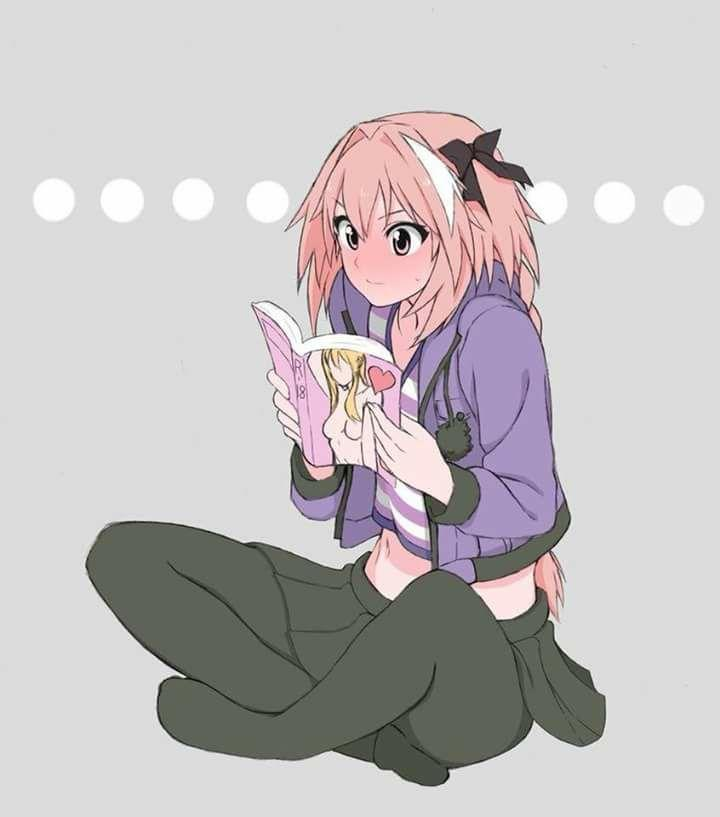
\includegraphics[width = 90mm]{figures/Astolfo_reading.jpg}
        }
    \end{figure*}
